\qrchapter{https://forgottenpillar.com/rsc/en-fp-chapter8}{The constructive criticism}


\qrchapter{https://forgottenpillar.com/rsc/en-fp-chapter8}{Ukosoaji wa kujenga}


The first point of the \emcap{Fundamental Principles} answers the questions: who is God, what is His personality, and how do we understand His presence?


Jambo la kwanza la \emcap{Kanuni za Msingi} hujibu maswali: Mungu ni nani, ni nini \emcap{Umbile} Wake, na tunaelewaje uwepo Wake?


\others{I. That there is \textbf{one God}, \textbf{a personal, spiritual }\textbf{\underline{being}}, \textbf{the creator of all things}, omnipotent, omniscient, and eternal; infinite in wisdom, holiness, justice, goodness, truth, and mercy; unchangeable, and \textbf{everywhere present by his representative, the Holy Spirit}. Ps. 139:7.}[FP1889 147.2; 1889][https://egwwritings.org/read?panels=p931.6]


\others{I. Kwamba kuna \textbf{Mungu mmoja}, \textbf{huluki binafsi wa kiroho}, \textbf{\underline{huluki}}, \textbf{Muumba wa vitu vyote}, mwenye uwezo wote, anayejua yote, na wa milele; Asiye na kikomo katika hekima, utakatifu, haki, wema, ukweli, na rehema; asiyebadilika, na \textbf{kila mahali akiwepo kwa mbinu ya mwakilishi wake, Roho Mtakatifu}. Zab. 139:7.}[FP1889 147.2; 1889][https://egwwritings.org/read?panels=p931.6]


The one God, the Creator, is identified as the Father, because the second point of the \emcap{Fundamental Principles} states that Jesus Christ, the Son of the Eternal Father, is the one by whom God created all things\footnote{\href{https://egwwritings.org/?ref=en_FP1889.147.3&para=931.7}{FP1889 147.3; 1889}}. The \emcap{personality of God} is expressed in the term “\textit{personal spiritual being}”. We will soon see that this term denotes that the Father has a material body, a physical manifestation. Thus, in His personality, He is present only where He dwells physically. But, His presence is not constrained to His personality because He is \others{everywhere present by his representative, the Holy Spirit}. During our past history, this understanding and reasoning of the \emcap{personality of God}, as expressed in the first point of the \emcap{Fundamental Principles}, received constructive criticism; by “constructive criticism” we refer to the criticism supported by the Bible.


Mungu mmoja, Muumba, anatambulika kama Baba, kwa sababu jambo la pili la \emcap{Kanuni za Msingi} linasema kwamba Yesu Kristo, Mwana wa Baba wa Milele, ndiye pekee ambaye Mungu aliumba vitu vyote\footnote{\href{https://egwwritings.org/?ref=en_FP1889.147.3&para=931.7}{FP1889 147.3; 1889}}. \emcap{Umbile la Mungu} unaonyeshwa katika neno “\textit{huluki binafsi wa kiroho}”. Hivi karibuni tutaona kwamba neno hili linamaanisha kwamba Baba ana mwili wa kimwili, udhihirisho wa kimwili. Kwa hivyo, katika Umbile Lake, Yeye yuko pale tu Anapokaa kimwili. Lakini, Uwepo Wake hauzuiliwi kwa Umbile Lake kwa sababu Yeye \others{yupo kila mahali kupitia mwakilishi wake, Roho Mtakatifu}. Wakati wa historia yetu iliyopita, ufahamu huu na hoja ya \emcap{Umbile la Mungu}, kama inavyoonyeshwa katika nukta ya kwanza ya \emcap{Kanuni za Msingi}, kulipokea ukosoaji wa kujenga; kwa “ukosoaji unaojenga” tunarejelea ukosoaji unaoungwa mkono na Biblia.


We now present to you the following citations, some constructive criticism, from a prominent trinitarian brother in the Seventh-day Adventist world. Interestingly, he had acknowledged the authority of the \emcap{Fundamental Principles}, yet simultaneously believed in the Trinity doctrine. We find this document a very important element in the change of our beliefs from the fundamental principles to current Seventh-day Adventist Trinitarian belief.


Sasa tunakuletea manukuu yafuatayo, ukosoaji fulani wenye kujenga, kutoka kwa ndugu mashuhuri katika shirika la Waadventista Wasabato. Inashangaza, alikuwa amekubali mamlaka ya \emcap{Kanuni za Msingi}, lakini wakati huo huo aliamini mafundisho ya utatu. Tunaona waraka huu kuwa kipengele muhimu sana katika mabadiliko ya imani zetu kutoka kanuni za msingi kuelekea kwa imani ya sasa ya Utatu wa Waadventista Wasabato.


This prominent brother was met with the question, “\textit{Do you not believe in a personal, definite God?}”:


Ndugu huyu mashuhuri alikutanishwa na swali, “\textit{Je, unaamini katika Mungu binafsi, aliye dhahiri?}”:


\others{\textbf{Most certainly. An infinite, divine, personal being is essential religion}. Worship requires someone to love, to obey, to trust. \textbf{Belief in a personal God is the very core of the Christian religion}. The conception of God as the All-Energy, the infinite Power, an all-pervading Presence, is too vast for the human mind to grasp; there must be something more \textbf{tangible}, more \textbf{\underline{restricted}}, upon which to center the mind in worship. \textbf{It is for this reason that Christ came to us in the image of God's }\textbf{\underline{personality}}\textbf{, the second Adam, to show us by his life of love and self-sacrifice the character and }\textbf{\underline{the personality of God}}. We can approach God only through Christ.}


\others{\textbf{Hakika. Huluki usio na mwisho, na wa kimungu, vilevile wa kibinafsi ni dini muhimu}. Ibada inahitaji Nafsi wa kumpenda, kutii, na kuamini. \textbf{Imani katika Mungu wa kibinafsi ndio msingi wa dini ya Kikristo}. Dhana ya Mungu kama Nishati-Yote, Nguvu isiyo na kikomo, Uwepo unaoenea kote, ni kubwa sana kwa akili ya mwanadamu kushika; lazima kuna kitu \textbf{inayoshikika} zaidi, \textbf{\underline{iliyowekewa vikwazo}} zaidi, ambayo kwayo akili itaegemea katika ibada. \textbf{Ni kwa sababu hii ndiposa Kristo alikuja kwetu kwa mfano wa }\textbf{\underline{Umbile}} \textbf{wa Mungu, Adamu wa pili, ili atuonyeshe kwa maisha yake ya upendo na ya kujitolea tabia na }\textbf{\underline{Umbile la Mungu}}. Tunaweza kumkaribia Mungu kupitia Kristo pekee.}


\othersnogap{‘Who being the brightness of his glory, and \textbf{the express image of his person}, and upholding all things by the word of his power, when he had by himself purged our sins, sat down on the right hand of the Majesty on high.’}


\othersnogap{‘Ambaye kwa kuwa ni mng'ao wa utukufu wake, na \textbf{chapa halisi ya nafsi yake}, na akivichukua vyote kwa neno la uweza wake, akiisha kufanya utakaso wa dhambi, akaketi chini kwenye mkono wa kuume wa Ukuu huko juu.’}


\othersnogap{‘Who being the effulgence of his glory, and the impress of his substance, and upholding all things by the word of his power.’}


\othersnogap{‘Ambaye kwa kuwa ni mng'ao wa utukufu wake, na chapa ya mali yake, na kuvichukua mambo yote kwa neno la uweza wake.’}


\othersnogap{The apostle says, ‘But we all, with open face \textbf{beholding as in a glass} the glory of the Lord, are changed into the same image from glory to glory, even as by the Spirit of the Lord.’ 2 Cor. 3: 18. How apt and beautiful is this figure!... So, \textbf{in beholding Christ} in his miracles, his temptations, his exhortations, his life of self-abnegation, his ‘going about doing good,’ \textbf{we may behold the personality and power of God}. And what a great hope there is for us in the fact that \textbf{in Christ we find qualities not strange and foreign to humanity}, but kindred mental and moral characteristics; so that we are able to see and grasp an actual, rather than merely a theological or abstract or figurative truth, in the declaration of the apostle, ‘Now are we the sons of God.’ 1 John 3:2.}


\othersnogap{Mtume asema, ‘Lakini sisi sote, kwa uso usiotiwa utaji, \textbf{tukiurudisha utukufu wa Bwana, kama vile katika kioo}, tunabadilishwa tufanane na mfano uo huo, toka utukufu hata utukufu, kama vile kwa Roho wa Bwana.’ 2 Kor. 3:18. Jinsi sura hii inavyofaa na ya kupendeza!... Kwa hiyo, \textbf{katika kumtazama Kristo} katika miujiza yake, majaribu, mawaidha yake, maisha yake ya kujinyima, ‘kuzunguka-zunguka akitenda mema,’ \textbf{tunaweza kuona Umbile na nguvu za Mungu}. Na kuna tumaini kubwa kiasi kipi kwetu katika ukweli kwamba \textbf{kwa Kristo tunapata sifa ambazo si ngeni na si za kukosa uwiano na za wanadamu}, bali sifa zenye ujamaa moja nasi kiakili na maadili; ili tuweze kuona na kufahamu jambo halisi, badala tu ya ukweli wa kitheolojia au wa kufikirika au wa mfano, katika tamko la mtume, ‘Sasa sisi wana wa Mungu.’ 1 Yohana 3:2.}


\othersnogap{\textbf{The fact that God is so great that we cannot form a clear mental picture of his }\textbf{\underline{physical appearance}}\textbf{ need not lessen in our minds the reality of }\textbf{\underline{His personality}}\textbf{, neither does this conception disagree with that of a special expression of God in some }\textbf{\underline{particular form or place}}. \textbf{\underline{Indeed, there are scriptures which present God in this definite, and one may say circumscribed, form as sitting upon a throne in heaven, or as dwelling in the temple at Jerusalem}}, 1. Kings 22:19; Ps. 11:4; Matt. 21:12, 13.}


\othersnogap{\textbf{Ukweli kwamba Mungu ni mkuu sana hivi kwamba hatuwezi kuwazia waziwazi akilini mwonekano wa }\textbf{\underline{kimwili}}\textbf{ hauhitaji kupunguza katika akili zetu ukweli wa }\textbf{\underline{Umbile Lake}}\textbf{, wala dhana hii haikubaliani na ile ya usemi maalum wa Mungu katika }\textbf{\underline{fomu fulani au mahali fulani}}. \textbf{\underline{Hakika yapo maandiko yanayomtambulisha Mungu katika umbo dhahiri, na mtu anaweza kusema njia ya kuzuiliwa, kama kuketi juu ya kiti cha enzi mbinguni, au kama akikaa katika hekalu la Yerusalemu}}, 1. Wafalme 22:19; Zab. 11:4; Mt. 21:12, 13.}


\othersnogap{The human mind is finite and cannot grasp infinity. \textbf{We naturally desire to form a definite, clearly defined conception of the being whom we worship}. \textbf{The Bible supplies this human need as well as all other of our spiritual requirements, and }\textbf{\underline{in the fortieth chapter of Isaiah}}\textbf{ the prophet deals with this question of God's personal appearance in a marvelous way}. ‘O Jerusalem, that bringest good tiding, lift up thy voice with strength; lift it up, be not afraid; say unto the cities of Judah, \textbf{Behold your God}! He shall feed his flock like a shepherd: he shall gather the lambs in his arms, and carry them in his bosom.’}


\othersnogap{Akili ya mwanadamu ina kikomo na haiwezi kutafakari na kuelewa kisicho na kikomo. \textbf{Kwa kawaida tunatamani kuunda kwa uhakika, kwa dhana iliyofafanuliwa waziwazi ya huluki tunayemwabudu}. \textbf{Biblia inapatanisha hitaji hili la mwanadamu na vile vile mahitaji yetu mengine yote ya kiroho, na }\textbf{\underline{katika sura ya arubaini ya Isaya}}\textbf{ nabii anashughulikia swali hili la sura ya kibinafsi ya Mungu kwa namna ya ajabu}. ‘Ee Yerusalemu, uletao habari njema, paza sauti yako kwa nguvu; inueni, msiogope; iambie miji ya Yuda, \textbf{Tazameni, Mungu wenu}! Atalilisha kundi lake kama mchungaji: atawakusanya wana-kondoo mikononi mwake, na kuwachukua kifuani mwake.’}


\othersnogap{‘Who hath measured the waters in the hollow of \textbf{his hand}, and meted out heaven with the span, and comprehended the dust of the earth in a measure, and weighed the mountains in scales, and the hills in a balance? \textbf{To whom then will ye liken God?} \textbf{Or what likeness will ye compare unto him?} Have ye not known? have ye not heard? hath it not been told you from the beginning? have ye not understood from the foundations of the earth? \textbf{It is he that sitteth upon the circle of the earth}, and the inhabitants thereof are as grasshoppers; \textbf{that stretcheth out the heavens as a curtain, and spreadeth them out as a tent to dwell in}: \textbf{\underline{To whom then will ye liken me, or shall I be equal? saith the Holy One}}. Lift up your eyes on high, and behold who hath created these things, that bringeth out their host by number: he calleth them all by names by the greatness of his might, for that he is strong in power; not one faileth. Hast thou not known? hast thou not heard, that the everlasting God, the Lord, the Creator of the ends of the earth, fainteth not, neither is weary? There is no searching of his understanding. He giveth power to the faint and to them that have no might he increaseth strength. Even the youths shall faint and be weary, and the young men shall utterly fall: but they that wait upon the Lord shall renew their strength; they shall mount up with wings as eagles; they shall run, and not be weary; and they shall walk, and not faint.’ Isa. 40:9,11,12,18,21,22,25,26,28-31.}


\othersnogap{‘Ni nani aliyepima maji katika tundu la \textbf{mkono wake}, na kuzipima mbingu kwa morita, na kuyashika mavumbi ya ardhi kwa kipimo, na kuyapima milima ndani ya mizani, na vilima katika mizani? \textbf{Mtamfananisha Mungu na nani basi?} \textbf{Au itakuwa mfano gani mnalinganisha naye?} Je! hamjui? hamjasikia? hamjaambiwa tangu mwanzo? hamjaelewa tangu kuwekwa misingi ya dunia? \textbf{Ni yeye huyo ameketi juu ya duara ya dunia}, na wakaaji wake ni kama panzi; \textbf{hivyo huzitandaza mbingu kama pazia, na kuzitandaza kama hema ya kukaa}: \textbf{\underline{Mtanifananisha na nani basi, au niwe sawa na nani? Asema Mtakatifu}}. Inua macho yako juu, na tazama, ni nani aliyeviumba hivi, yeye aletaye nje jeshi lao kwa hesabu; huwaita wote kwa majina kwa ukuu wa uweza wake, kwa kuwa ana nguvu katika uweza; sivyo mmoja hushindwa. Je, hukujua? hukusikia ya kwamba Mungu wa milele, Bwana, Muumba miisho ya dunia, hazimii wala hachoki? Hakuna kutafuta ufahamu wake. Huwapa nguvu wazimiao na kuwaongeza wasio na uwezo nguvu. Hata vijana watazimia na kuchoka, na vijana wataanguka, lakini wao wamngojeao Bwana watapata nguvu mpya; watapanda juu kwa mbawa kama tai; watapiga mbio, wala hawatachoka; watakwenda kwa miguu, wala hawatazimia.’ Isa. 40:9,11,12,18,21,22,25,26,28-31.}


\othersnogap{\textbf{Here is a most marvelous description of God. His hand, his arm, his bosom are mentioned}. He is described as ‘sitting on the circle of the earth,’ he metes out heaven with the span, he holds the waters in the hollow of his hand; \textbf{\underline{so there can be no question that God is a definite, real, personal being}}. \textbf{A mere abstract principle, a law, a force could not have a hand, an arm. \underline{God is a person}, though too great for us to comprehend, as Job says}, ‘God is great and we know him not.’ Job 36:26...}


\othersnogap{\textbf{Hapa kuna maelezo ya ajabu sana ya Mungu. Mkono wake, mkono wake, kifua chake zinatajwa}. Anafafanuliwa kuwa ‘ameketi juu ya duara ya dunia,’ analinganisha mbingu kwa morita, huyashika maji katika tundu la mkono wake; \textbf{\underline{hivyo hakuwezi kuwa na swali kwamba Mungu ni huluki dhahiri, halisi na wa kibinafsi}}. \textbf{Kanuni ya kufikirika tu, sheria, nguvu hawezi kuwa na viganja au mkono. \underline{Mungu ni Nafsi}, ingawa ni mkuu sana kwetu sisi kuelewa, kama Ayubu anasema}, ‘Mungu ni mkuu na sisi hatumjui.’ Ayubu 36:26...}


\othersnogap{\textbf{\underline{This great being} is represented as sitting on the circle of the earth}. The orbit of the earth is nearly two hundred million miles in diameter. \textbf{A being so great as to occupy a seat of such proportions is quite \underline{beyond our comprehension as regards his form}}. \textbf{The prophet recognizes this, and so \underline{diverts our attention away from speculation respecting the exact size and form of God} by showing us the absurdity of trying to form even a mental image, \underline{intimating that this is closely akin to idolatry}. See verses 18-21}. He then shows us where to find a true conception of God, pointing us to the things which he has made: ‘Lift up your eyes on high and behold who hath created these things.’ This also was Paul's idea : ‘For the invisible things of him from the creation of the world are clearly seen, being understood by the things that are made, \textbf{even his eternal power and \underline{Godhead}}; so that they are without excuse.’ Rom. 1:20.}


\othersnogap{\textbf{\underline{Huluki huyu mkubwa} Anawakilishwa kama ameketi kwenye duara la dunia}. Mzunguko wa dunia ina kipenyo cha takriban maili milioni mia mbili. \textbf{Huluki mkubwa sana hadi kuchukua kiti cha namna hiyo ni \underline{zaidi ya ufahamu wetu kuhusu umbo lake}}. \textbf{Nabii anatambua hili, na hivyo \underline{kugeuza mawazo yetu mbali na uvumi kuhusu ukubwa na umbo kamili wa Mungu} kwa kutuonyesha upuuzi wa kujaribu kufanyiza hata picha akilini, \underline{akionyesha kwamba jambo hilo ni sawa kabisa na ibada ya sanamu}. Tazama mistari 18-21}. Kisha anatuonyesha mahali pa kupata wazo la kweli la Mungu, akituelekeza kwenye mambo ambayo ameifanya: ‘Inueni macho yenu juu, mwone ni nani aliyeviumba hivi. Hili pia lilikuwa wazo la Paulo: ‘Kwa maana vitu vyake visivyoonekana tangu kuumbwa ulimwengu vinaonekana waziwazi, ikifahamika kwa vitu vilivyofanyika, \textbf{yaani, uweza wake wa milele na \underline{Uungu}}; ili wasiwe na udhuru.’ Rum. 1:20.}


\othersnogap{\textbf{\underline{Discussions respecting the form of God are utterly unprofitable}, and serve only to belittle our conceptions of him who is above all things}, \textbf{and hence not to be compared in form or size or glory or majesty with anything which man has ever seen or which it is within his power to conceive}. In the presence of questions like these, we have only to acknowledge our foolishness and incapacity, and bow our heads with awe and reverence \textbf{in the presence of a Personality, an Intelligent Being} to the existence of which all nature bears definite and positive testimony, \textbf{but which is as far beyond our comprehension \underline{as are the bounds of space and time}}.}


\othersnogap{\textbf{\underline{Majadiliano yanayohusu umbo la Mungu hayana faida kabisa}, na hutumikia tu kudhalilisha dhana zetu za yeye aliye juu ya vitu vyote}, \textbf{na hivyo haipaswi kulinganishwa kwa umbo au ukubwa au utukufu au ukuu pamoja na kitu chochote ambacho mwanadamu amewahi kukiona au ambacho kicho katika uwezo wake kuuvutia taswira}. Katika uwepo wa maswali kama haya, lazima tu tukiri upumbavu wetu na kutoweza, na tuinamishe vichwa vyetu kwa kicho na heshima \textbf{mbele ya uwepo wa Nafsi, Huluki wenye Akili} uwepo wake ambao kwayo maumbile yote ina ushuhuda wa uhakika na chanya, \textbf{lakini ambaye ni mbali zaidi ya uwezo wa ufahamu wetu \underline{kama vile mipaka ya nafasi na wakati}}.}


As mentioned before, this brother acknowledges the \emcap{Fundamental Principles}, yet believes in the Trinity. Here is a short summary of His constructive criticism regarding the \emcap{personality of God}: God is a definite, real, personal being, having a form—\others{\textbf{Indeed, there are scriptures which present God in \underline{this definite}, and one may say \underline{circumscribed}, form as sitting upon a throne in heaven}}. He advocates this because he believes it is necessary for us, finite human beings, to have a definite object of worship. But he expands the idea of a “\textit{circumscribed} God by the testimony from Isaiah chapter 40, which proves that God is\others{\textbf{\underline{beyond our comprehension as regards his form}}}. Any kind of conceptualization of God’s being, in any form, is akin to idolatry. \others{\textbf{\underline{Discussions respecting the form of God are utterly unprofitable}}}. The true matter of the personality of infinite God is beyond our comprehension. God’s true personality is more than a mystery to our finite minds. This is because God is\others{\textbf{far beyond our comprehension \underline{as are the bounds of space and time}}}. For this brother, understanding God’s personality merely as a definite being is in one way true, but in another way false. It is true that God presented Himself in \others{\textbf{\underline{particular form or place}}}, because \others{there must be something more \textbf{tangible}, more \textbf{\underline{restricted}}, upon which to center the mind in worship}. A simple understanding of God as a definite and tangible being is restrictive for God. The summary of his criticism is that we should form our conceptions of God outside of \others{\textbf{the bounds of space and time}}.


Kama ilivyotajwa hapo awali, ndugu huyu anakubali \emcap{Kanuni za Msingi}, lakini analiamini Utatu. Huu hapa ni muhtasari mfupi wa ukosoaji Wake wenye kujenga kuhusu \emcap{ubinafsi wa Mungu}: Mungu ni huluki dhahiri, halisi, binafsi, mwenye umbo—\others{\textbf{Hakika, kuna maandiko ambayo yanamwasilisha Mungu katika \underline{hali hii ya umbo dhahiri}, na mtu anaweza kusema njia ya \underline{kuzuiliwa}, kama ameketi juu ya kiti cha enzi mbinguni}}. Anatetea hili kwa sababu anaamini ni muhimu kwetu, wanadamu wenye ukomo, kuwa na shabaha ya hakika ya kuabudiwa. Lakini anapanua wazo la Mungu “aliyezuiliwa” kwa ushuhuda kutoka kwa Isaya sura ya 40, ambayo inathibitisha kwamba Mungu yuko\others{\textbf{\underline{zaidi ya ufahamu wetu kuhusu umbo lake}}}. Aina yoyote ya dhana ya Mungu kuwa, kwa namna yoyote ile, ni sawa na ibada ya sanamu. \others{\textbf{\underline{Majadiliano yanayohusu umbo la Mungu hayana faida kabisa}}}. Jambo la kweli la ubinafsi wa Mungu asiye na kikomo ni zaidi ya ufahamu wetu. Ubinafsi wa kweli wa Mungu ni zaidi ya fumbo kwa akili zetu zenye kikomo. Hii ni kwa sababu Mungu yuko\others{\textbf{mbali zaidi ya uwezo wa ufahamu wetu \underline{kama vile mipaka ya nafasi na wakati}}}. Kwa ndugu huyu, kuelewa ubinafsi wa Mungu kama Huluki hususa ni kwa njia moja kweli, lakini kwa njia nyingine ni uwongo. Ni kweli kwamba Mungu alijidhihirisha katika \others{\textbf{\underline{fomu au mahali maalum}}}, kwa sababu \others{lazima kuwe na kitu \textbf{kinachoonekana} zaidi, \textbf{\underline{kilichozuiliwa}} zaidi, ambacho kinaweza tegemeza akili katika ibada}. Ufahamu nyepesi wa Mungu kama huluki dhahiri na wa kushikika ni kizuizi kwa Mungu. Muhtasari wa ukosoaji wake ni kwamba tunapaswa kuunda dhana zetu za Mungu nje ya \others{\textbf{mipaka ya nafasi na wakati}}.


Please, candidly examine the reasons behind this brother’s faith. The reasoning behind his arguments is important to understand because it played an important role in Seventh-day Adventist history, as a bold step away from the \emcap{Fundamental Principles}. These arguments are not trivial; they are very persuasive and we urge you to their contemplation. Perhaps you might agree with them, but please allow us to unmask the deception. These citations are from Dr. Kellogg’s book “\textit{The Living Temple}”\footnote{\href{https://archive.org/details/J.H.Kellogg.TheLivingTemple1903}{Dr. J. H. Kellogg, The Living Temple, p.29-33.}}. From the section titled “\textit{Infinite Intelligence a Personal being}”, pages 29 to 33, the passages express Kellogg’s position on the \emcap{personality of God}, which was the main problem with his book.


Tafadhali, chunguza kwa unyoofu sababu za imani ya ndugu huyu. Mwongozo wa fikira zake ni muhimu kuuelewa kwa sababu ulichukua jukumu muhimu katika Historia ya Waadventista Wasabato, kama hatua ya ujasiri mbali na \emcap{Kanuni za Msingi}. Hoja hizi sio ndogo; unao ushawishi sana na tunakuhimiza utafakari. Labda wewe unaweza kukubaliana nao, lakini tafadhali turuhusu kufichua udanganyifu. Nukuu hizi ni kutoka kwa kitabu cha Dk. Kellogg “The Living Temple”\footnote{\href{https://archive.org/details/J.H.Kellogg.TheLivingTemple1903}{Dr. J. H. Kellogg, The Living Temple, p.29-33.}}. Kutoka kwa sehemu yenye kichwa “Huluki Binafsi Aliye na Ujuzi Bila Kikomo”, ukurasa wa 29 hadi 33, vifungu vinaeleza msimamo wa Kellogg kuhusu \emcap{ubinafsi wa Mungu}, ambalo lilikuwa tatizo kuu la kitabu chake.


That which you just read was exactly what Sister White referred to when she said: \egwinline{I have some things to say to our teachers \textbf{in reference to the new book The Living Temple}. \textbf{Be careful how you sustain the sentiments of this book \underline{regarding the personality of God}}. As the Lord presents matters to me, \textbf{these sentiments do not bear the endorsement of God}. \textbf{They are a snare that the enemy has prepared for these last days}...}[Lt211-1903.1; 1903][https://egwwritings.org/read?panels=p9598.8]


Hicho ambacho umesoma hivi punde ndicho hasa Dada White alirejelea aliposema: \egwinline{Ninao mambo machache ya kusema kwa walimu wetu \textbf{yakirejelea kitabu kipya The Living Temple}. \textbf{Kuwa mwangalifu jinsi unavyotegemeza hisia za kitabu hiki \underline{kuhusu ubinafsi wa Mungu}}. Bwana anavyowasilisha mambo kwangu, \textbf{hisia hizi hazikubaliki na Mungu}. \textbf{Ni mtego ambao adui ameutayarisha kwa siku hizi za mwisho}...}[Lt211-1903.1; 1903][https://egwwritings.org/read?panels=p9598.8]


In the present Seventh-day Adventist controversy over the Trinity doctrine, we have personally been trying to shift the controversy from the Trinity doctrine to the \emcap{personality of God}. We’ve presented the position of the first point of the \emcap{Fundamental Principles} and have encountered arguments that greatly overlap with Dr. Kellogg’s sentiment on the \emcap{personality of God}, advocated in “\textit{Living Temple}”. We’ve seen this repeatedly. When the focus is drawn from the Trinity issue to the \emcap{personality of God}, Kellogg’s views regarding the \emcap{personality of God} frequently echoe from the lips of Trinitarian advocates. The quality or state of God being a person is a mystery in the Trinity doctrine, and often Kellogg’s sentiment on the \emcap{personality of God} resonates with Trinitarian understanding of God’s person.


Katika pambano la sasa la Waadventista Wasabato juu ya fundisho la Utatu, kibinafsi tumekuwa tukijaribu kuhamisha utata kutoka kwa fundisho la Utatu hadi \emcap{ubinafsi wa Mungu}. Tumewasilisha msimamo wa hoja ya kwanza ya \emcap{Kanuni za Msingi} na tumekumbana na mabishano ambayo yanaingiliana sana na maoni ya Dk. Kellogg juu ya \emcap{ubinafsi wa Mungu}, yanayotetewa katika “The Living Temple”. Tumeona hili mara kwa mara. Wakati umakini unatolewa kutoka kwa suala la Utatu hadi \emcap{ubinafsi wa Mungu}, maoni ya Kellogg kuhusu \emcap{ubinafsi wa Mungu} mara kwa mara hutoka midomoni mwa watetezi wa Utatu. Ubora au hali ya Mungu kuwa Nafsi ni fumbo katika fundisho la Utatu, na mara nyingi maoni ya Kellogg juu ya \emcap{ubinafsi wa Mungu} inapatana na ufahamu wa Utatu wa nafsi ya Mungu.


\begin{figure}[hp]
    \centering
    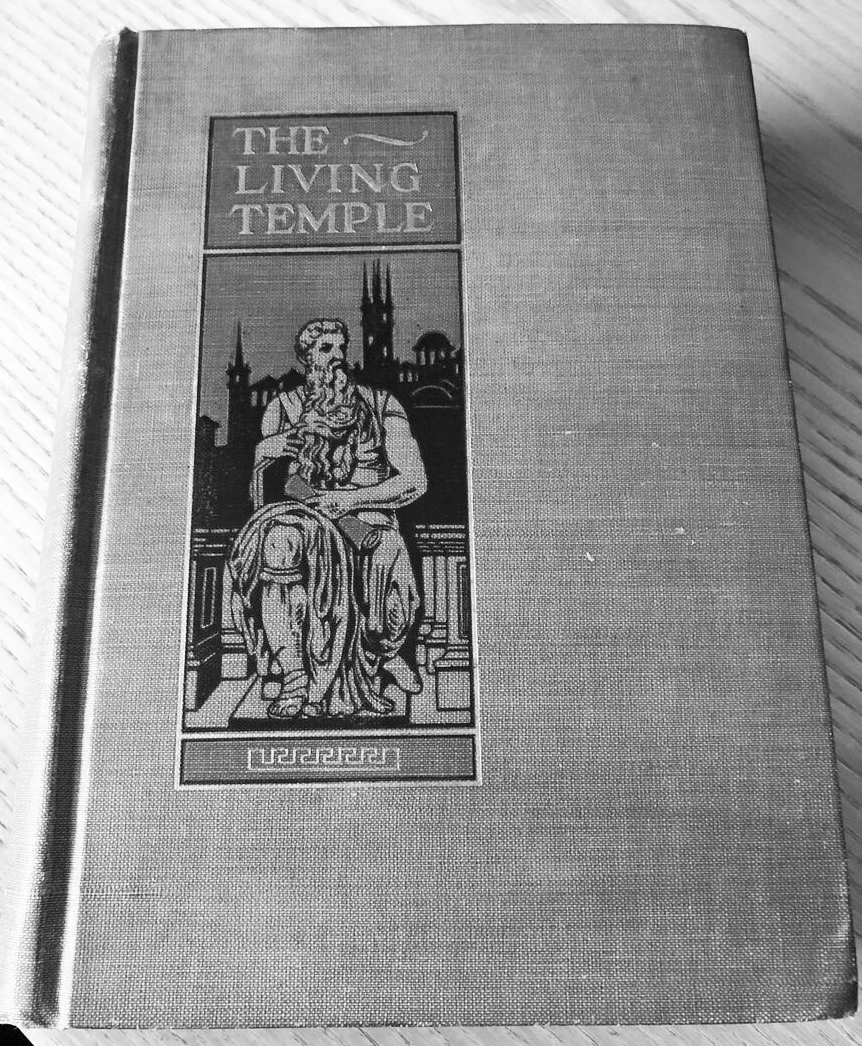
\includegraphics[width=1\linewidth]{images/TLT.jpg}
    \caption*{The Living Temple by Dr. J. H. Kellogg, 1903}
    \label{fig:tlt}
\end{figure}


\begin{figure}[hp]
    \centering
    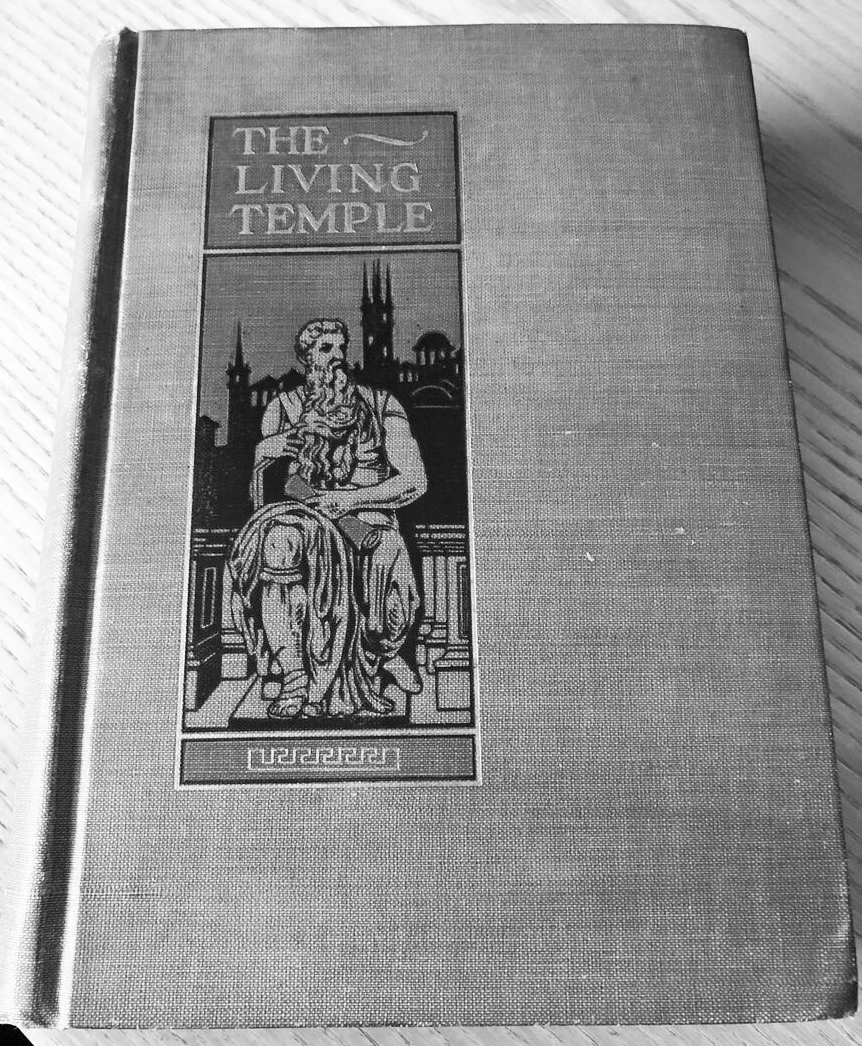
\includegraphics[width=1\linewidth]{images/TLT.jpg}
    \caption*{The Living Temple na Dk. J. H. Kellogg, 1903}
    \label{fig:tlt}
\end{figure}


Some people find Dr. Kellogg’s understanding of God’s personality resonates with their understanding, yet they are tempted to think that there are other things objectionable with the Living Temple. The following evidence suggests the very opposite. There is a letter from Dr. Kellogg to William C. White, where Dr. Kellogg proposes to \others{cutting out a few leaves} from the three thousand copies of the Living Temple—those very leaves containing the \others{specially objectionable things appear, such as the comment on Isaiah 40} and the sentiments regarding the \emcap{personality of God} (the pages we have read).


Baadhi ya watu wanaona ufahamu wa Dk. Kellogg kuhusu Umbile la Mungu unahusiana na uelewa wao, lakini wanashawishika kufikiri kwamba kuna mambo mengine ya kukemewa zaidi katika Hekalu Hai. Ushahidi ufuatao unaonyesha kinyume kabisa. Kuna barua kutoka Dk. Kellogg kwa William C. White, ambapo Dk. Kellogg anapendekeza \others{kukatwa kwa kurasa chache} kutoka kwa nakala elfu tatu za Hekalu Hai—kurasa zile zenye \others{hasa mambo yenye kuchukiza yanatokea, kama vile maelezo juu ya Isaya 40} na maoni kuhusu \emcap{Umbile la Mungu} (kurasa ambazo tumesoma).


\others{The Sanitarium has on hand, I find, \textbf{two or three thousand books which were sold}, but which have come back since the book was condemned. The question has been raised, what shall be done with these? \textbf{It has occurred to me that perhaps they might be saved \underline{by cutting out a few leaves} in which the \underline{specially objectionable things appear}, such as the \underline{comment on Isaiah 40}, which I borrowed from A.T. Jones, and the page on which the unfortunate heading appears, ‘\underline{The Personality of God},’ and tipping in leaves embodying a clear statement of the Bible view of God as a person presented in Elder Haskell’s article in the ‘Review’ a few weeks ago}. These books would be sold to old patients who are making a great demand for the book for Christmas presents…}[Letter from Dr. J.H. Kellogg to W.C.White; December 6, 1903, Chicago][https://174625.selcdn.ru/ellenwhite/EWhite/17226/17226.pdf]


\others{Sanitarium iko nazo, napata, \textbf{vitabu elfu mbili au elfu tatu ambavyo viliuzwa}, lakini ambavyo vimeregeshwa tangu kitabu kilipokaripiwa. Swali limeulizwa, je! Nini kitafanywa na hivi? \textbf{Wazo limenijia kwamba labda vinaweza kuokolewa \underline{kwa kukata kurasa chache} ambazo \underline{hasa mambo yenye kuchukiza yanatokea}, kama vile \underline{maoni juu ya Isaya 40}, ambayo nilikopa kutoka kwa A.T. Jones, na ukurasa ambao kichwa cha bahati mbaya kinaonekana, ‘\underline{Umbile la Mungu},’ na kupeana kurasa zinazojumuisha taarifa iliyo wazi ya maoni ya Biblia juu ya Mungu kama Nafsi inayotolewa katika Nakala ya Mzee Haskell katika ‘Review’ wiki chache zilizopita}. Vitabu hivi vitauzwa kwa wazee wagonjwa wanaohitaji sana kitabu cha zawadi za Krismasi…}[Letter from Dr. J.H. Kellogg to W.C.White; December 6, 1903, Chicago][https://174625.selcdn.ru/ellenwhite/EWhite/17226/17226.pdf]


What is the real issue with the reasoning in the Living Temple? We will study the matter to its very depth; superficially, we clearly see that the issue is the stepping off of the foundation of our faith—the \emcap{Fundamental Principles}—regarding the \emcap{personality of God} and where His presence is.


Je, ni suala gani la kweli kuhusu hoja zilizowasilishwa katika Hekalu Hai? Tutajifunza suala hilo hadi kwenye mizizi yake; kijuujuu, tunaona wazi kuwa suala ni kuvuka msingi wa imani yetu—\emcap{Kanuni za Kimsingi}—kuhusu \emcap{Umbile la Mungu} na mahali uwepo wake upo.


\egw{\textbf{I have been instructed by the heavenly messenger} that \textbf{some of the reasoning} in the book, ‘Living Temple’, is unsound and that \textbf{this reasoning would lead astray} the minds of those who are not thoroughly established on \textbf{the foundation principles} of present truth. \textbf{It introduces that which is naught but speculation} in \textbf{regard to the personality of God and where His presence is}.}[SpTB02 51.3; 1904][https://egwwritings.org/read?panels=p417.262]


\egw{\textbf{Nimeagizwa na mjumbe wa mbinguni} kwamba \textbf{baadhi ya hoja} katika kitabu, ‘Hekalu Hai’, hazina msimamo wa kweli na kwamba \textbf{mawazo haya yangepotosha} akili za wale ambao hawajaimarishwa kikamilifu kuhusu \textbf{kanuni za msingi} za ukweli wa sasa. \textbf{Inatanguliza yale ambayo si kitu ila dhana tu} kuhusiana na \textbf{Umbile la Mungu na uwepo wake ulipo}.}[SpTB02 51.3; 1904][https://egwwritings.org/read?panels=p417.262]


Dr. Kellogg introduced the thought \egwinline{which is naught but speculation in regard to the personality of God}, by which he stepped off of the foundation of our faith—the \emcap{Fundamental Principles}. Discordance between Dr. Kellogg’s teaching and the \emcap{Fundamental Principles} is in the first statement of the principles where we are taught that\others{That there is \textbf{one God}, \textbf{a personal, spiritual \underline{being}}, \textbf{the creator of all things}, ... and \textbf{everywhere present by his representative, the Holy Spirit}. Ps. 139:7.}


Dk. Kellogg alianzisha wazo \egwinline{ambalo si lolote bali ni uvumi kuhusu Umbile la Mungu}, ambayo kwayo alivuka na kutoka kwenye msingi wa imani yetu—\emcap{Kanuni za Kimsingi}. Tofauti kati ya mafundisho ya Dk. Kellogg na \emcap{Kanuni za Kimsingi} iko katika kauli ya kwanza ya kanuni ambapo tunafundishwa kwamba\others{Kwamba kuna \textbf{Mungu mmoja}, \textbf{huluki binafsi wa kiroho}, \textbf{muumba wa vitu vyote}, ... na \textbf{kila mahali kiwepo na wake mwakilishi, Roho Mtakatifu}. Zab. 139:7.}


Sister White directly warned us of the sentiments expressed in the Living Temple regarding the \emcap{personality of God}. They are not in harmony with the first point of the \emcap{Fundamental Principles}, which were part of the foundation of our faith.


Dada White alituonya moja kwa moja kuhusu maoni yaliyoonyeshwa katika Hekalu Hai kuhusu \emcap{Umbile la Mungu}. Hazipatani na hoja ya kwanza ya \emcap{Kanuni za Kimsingi}, ambayo yalikuwa sehemu ya msingi wa imani yetu.


\egw{\textbf{I have had to write much concerning the strange doctrines and theories expressed in Living Temple. \underline{Were these theories accepted by our people, the strong pillars of our faith and the truths that have made Seventh-day Adventists what they are would be swept away}. I have had to show the fallacy of these doctrines, presenting them \underline{as a species of last-day heresy}. We are told by the Word of God that just such teaching \underline{will be brought in at this time}.}}[Lt250-1903.2; 1903][https://egwwritings.org/read?panels=p9337.8]


\egw{\textbf{Nimelazimika kuandika mengi kuhusu mafundisho ya ajabu na nadharia zinazoonyeshwa katika Hekalu Hai. \underline{Ikiwa nadharia hizi zingekubaliwa na watu wetu, nguzo imara za imani yetu na kweli ambazo zimetuwafanya Waadventista Wasabato jinsi walivyo zingefagiliwa mbali}. Nimelazimika kuonyesha uwongo wa mafundisho haya, nikiyawasilisha \underline{kama aina za uzushi wa siku za mwisho}. Tunaambiwa kwa Neno la Mungu kwamba mafundisho kama hayo \underline{yataletwa ndani hasa kwa wakati huu}.}}[Lt250-1903.2; 1903][https://egwwritings.org/read?panels=p9337.8]


Today we witness the widespread acceptance of Kellogg’s theories regarding the \emcap{personality of God}. The fact that the first point of the \emcap{Fundamental Principles} is no longer present in our beliefs proves that Kellogg’s theories regarding the \emcap{personality of God} have had an influence in shaping our beliefs.


Leo tunashuhudia kukubalika kwa nadharia za Kellogg kuhusu \emcap{Umbile la Mungu}. Ukweli kwamba hatua ya kwanza ya \emcap{Kanuni za Kimsingi} haipo tena katika imani yetu inathibitisha kwamba nadharia za Kellogg kuhusu \emcap{Umbile la Mungu} zimekuwa na ushawishi katika kutengeneza imani zetu.


\egw{One and another come to me, asking me to \textbf{explain the positions taken in “Living Temple.”} I reply, “They are unexplainable.” \textbf{The sentiments expressed do not give a true knowledge of God.} \textbf{All through the book are passages of scripture}. \textbf{These scriptures are brought in in such a way \underline{that error is made to appear as truth}}. \textbf{Erroneous theories are presented in so pleasing a way that unless care is taken, many will be misled}.}[SpTB02 52.1; 1904][https://egwwritings.org/read?panels=p417.265]


\egw{Mmoja na mwingine wanakuja kwangu, wakiniuliza \textbf{nieleze nafasi zilizochukuliwa katika “Hekalu Hai.”} Ninajibu, “Hazielezeki.” \textbf{Maoni yanayotolewa hayatoi ukweli kuhusu maarifa ya Mungu.} \textbf{Katika kitabu chote kuna vifungu vya maandiko}. \textbf{Maandiko haya yanaletwa kwa njia ambayo \underline{kosa linafanywa lionekane kuwa kweli}}. \textbf{Nadharia potofu zinawasilishwa kwa njia ya kupendeza sana hivi kwamba isipokuwa uangalifu unachukuliwa, wengi watapotoshwa}.}[SpTB02 52.1; 1904][https://egwwritings.org/read?panels=p417.265]


The error is being made to appear as truth, and many are misled.


Kosa linafanywa lionekane kuwa kweli, na wengi wamepotoshwa.


It is worth emphasizing, for some careless reader, that the real issue of Dr. Kellogg, and his book “\textit{Living Temple}”, is not the Trinity but the small step he took off of the \emcap{Fundamental Principles}. In order to understand the real issue of his book, it would be wrong to focus on its overlapping sentiments with the Trinity doctrine. Rather, we should focus on the point that constituted this small step he made; and this includes having a deep understanding of the \emcap{fundamental principles} just as our pioneers had. Who better to ask than the Adventist pioneers themselves?


Inafaa kusisitiza, kwa msomaji fulani asiyemakinika, kwamba suala halisi la Dk. Kellogg, na kitabu chake “\textit{Living Temple}”, si Utatu bali ni hatua ndogo aliyoichukua kutoka kwenye \emcap{Kanuni za Msingi}. Ili kuelewa suala halisi la kitabu chake, itakuwa ni makosa kuzingatia hisia zake zinazopishana na fundisho la Utatu. Badala yake, tunapaswa kuzingatia jambo hilo likijumuisha hatua hii ndogo aliyoichukua; na hii ni pamoja na kuwa na uelewa wa kina wa \emcap{kanuni za msingi} kama vile waanzilishi wetu walivyokuwa. Nani bora kuuliza isipokuwa Waadventista waanzilishi wenyewe?


% Constructive Criticism

\begin{titledpoem}
    
    \stanza{
        A personal God in heaven sits enthroned, \\
        This truth in our Principles firmly zoned. \\
        Present everywhere by Spirit's might, \\
        This foundation stood as our guiding light.
    }

    \stanza{
        Then came words that seemed so wise and deep, \\
        A subtle shift that made the faithful weep. \\
        "God's form beyond all human thought," they claimed, \\
        A mystery too vast to be contained or named.
    }

    \stanza{
        "Discussions of God's form," the Temple said, \\
        "Are futile paths where idols lie ahead." \\
        Yet this philosophy so smoothly spun, \\
        Was the very snare by which souls were won.
    }

    \stanza{
        The error dressed as truth appeared so fair, \\
        As scripture twisted in a clever snare. \\
        One small step from the Principles we held, \\
        One giant leap by which our faith was felled.
    }

    \stanza{
        Beware the mind that thinks itself too wise, \\
        To see deception veiled in truth's disguise. \\
        God is personal, definite, and real, \\
        This is the truth the Temple would conceal. 
    }
\end{titledpoem}


% Constructive Criticism

\begin{titledpoem}
    
    \stanza{
        A personal God in heaven sits enthroned, \\
        This truth in our Principles firmly zoned. \\
        Present everywhere by Spirit's might, \\
        This foundation stood as our guiding light.
    }

    \stanza{
        Then came words that seemed so wise and deep, \\
        A subtle shift that made the faithful weep. \\
        "God's form beyond all human thought," they claimed, \\
        A mystery too vast to be contained or named.
    }

    \stanza{
        "Discussions of God's form," the Temple said, \\
        "Are futile paths where idols lie ahead." \\
        Yet this philosophy so smoothly spun, \\
        Was the very snare by which souls were won.
    }

    \stanza{
        The error dressed as truth appeared so fair, \\
        As scripture twisted in a clever snare. \\
        One small step from the Principles we held, \\
        One giant leap by which our faith was felled.
    }

    \stanza{
        Beware the mind that thinks itself too wise, \\
        To see deception veiled in truth's disguise. \\
        God is personal, definite, and real, \\
        This is the truth the Temple would conceal. 
    }
\end{titledpoem}
